\section{Applications and Results}
\label{sec:results}
%
In this section, we \sz{first provide experimental validations (\S\ref{subsec:res_validation})} and then showcase our method on a number of applications and demonstrate its effectiveness (\S\ref{subsec:res_main}).
All the renderings are generated using the Mitsuba physically based renderer~\cite{Mitsuba} with our layered model implemented as a BSDF plugin.
Please see the accompanying video for animated versions of several results.

\sz{
	All the multi-layer results in the paper use our bidirectional estimator with the explicit implementation (although our BSDF plugin also supports nesting BSDFs).
	This is because the former runs faster, as seen in Figure~\ref{fig:result_multilayer}-c.
}
% We currently use double precision floating point arithmetic in all results. 

\sz{

%\vspace{5mm}

\subsection{Validations}
\label{subsec:res_validation}

\subsubsection{Cross validation}
%\myparagraph{Cross validation}
In Figures~\ref{fig:hemispheres} and \ref{fig:pdf-validate} as well as the supplemental material, we cross-validate our Monte Carlo estimators depicted in \S\ref{subsec:ours_eval} by comparing our estimated BSDFs/pdfs to references generated using forward sampling (\S\ref{subsec:ours_sample}) and binning. Notice that the sampling procedure is a straightforward process that requires none of the complexity introduced by our path formulation and estimators.

\subsubsection{White furnace tests}
%\myparagraph{White furnace tests}
We conducted a few ``white furnace tests'' to demonstrate the energy conservation of our layered BSDFs (Figure~\ref{fig:whitetest}).
For all these examples, the BSDFs are constructed such that no energy is lost due to light-layer interactions.
Under constant lighting (where identical amount of light comes from all directions), the object becomes invisible, demonstrating that our layered BSDFs indeed conserve energy properly.
}

% White Furnace test figure
\begin{figure}[h]
	\addtolength{\tabcolsep}{-3.5pt}
	\begin{tabular}{ccc}
		\begin{overpic}[width=0.315\columnwidth]{img/validations/whitetest/sphere_layered_noMedium_env.jpg}
			\put(2,3){\bfseries \color{white} (a1)}
		\end{overpic}
		&
		\begin{overpic}[width=0.315\columnwidth]{img/validations/whitetest/sphere_layered_withMedium_env.jpg} 
			\put(2,3){\bfseries \color{white} (b1)}
		\end{overpic}	
		&
		\begin{overpic}[width=0.315\columnwidth]{img/validations/whitetest/plane_layered_env.jpg} 
			\put(2,3){\bfseries \color{white} (c1)}
		\end{overpic}
		\\
		\begin{overpic}[width=0.315\columnwidth]{img/validations/whitetest/sphere_layered_noMedium_const.jpg}
			\put(2,3){\bfseries (a2)}
		\end{overpic}
		&
		\begin{overpic}[width=0.315\columnwidth]{img/validations/whitetest/sphere_layered_withMedium_const.jpg}
			\put(2,3){\bfseries (b2)}
		\end{overpic}
		&
		\begin{overpic}[width=0.315\columnwidth]{img/validations/whitetest/plane_layered_const.jpg}
			\put(2,3){\bfseries (c2)}
		\end{overpic}
	\end{tabular}
	%
	\caption{\label{fig:whitetest}
		\sz{
			\textbf{White furnace tests.}
			We demonstrate that our BSDFs conserve energy properly via three layered BSDF examples respectively given by
			\textbf{(a)}~a dielectric and a diffuse interface;
			\textbf{(b)}~a dielectric and a conductor interface and participating medium;
			\textbf{(c)}~two dielectric interfaces and participating medium in between.
			All the interfaces and media have albedo one (so no energy is lost due to light-layer interactions).
			For each example, a simple object is rendered under both environmental~(1) and constant~(2) illuminations.
		}
	}
\end{figure}


\subsection{Main Results}
\label{subsec:res_main}

\subsubsection{Application: Coating thickness/normal variation}
%\myparagraph{Application: Coating thickness/normal variation}
%
Figure~\ref{fig:result_glints} shows renderings of a globe with a dielectric coating on top of a metallic substrate.
In this example, both interfaces are colorless and the layer medium has a blue tint.
In Figure~\ref{fig:result_glints}-a, both interfaces are smooth, creating two overlapped reflections of the environment map with different amounts of blur.
In Figure~\ref{fig:result_glints}-b, the top interface of the globe is smooth, leading to one clear reflection.
On the bottom (metallic) interface, we use a detailed height field to drive the normal variation as well as the medium thickness.
The high-frequency variation of normal direction has resulted in detailed highlights on the bottom surface.
Further, due to varying amounts of attenuation at different thickness, these highlights exhibit different colors: reflections from greater depths become darker and more saturated. 
In Figure~\ref{fig:result_glints}-c, the height variation is instead applied to the top dielectric interface, causing the clear reflection of the environment to be replaced by a blurred one.
Further, since the areas under the continents now have larger thickness, their colors become more saturated.
Our layered BSDF model is capable of producing all these appearances using a simple set of parameters (thickness, roughness and medium absorption) in conjunction with spatial variation.

\begin{figure*}[t]
	\centering
	\addtolength{\tabcolsep}{-3pt}
	\begin{tabular}{ccc}
		\begin{overpic}[width=0.32\textwidth]{img/results/glints_globe_none_combine.jpg}
			\put(2,3){\bfseries \large (a)}
		\end{overpic}
		&
		\begin{overpic}[width=0.32\textwidth]{img/results/glints_globe_bottom_combine.jpg}
			\put(2,3){\bfseries \large (b)}
		\end{overpic}
		&
		\begin{overpic}[width=0.32\textwidth]{img/results/glints_globe_top_combine.jpg}
			\put(2,3){\bfseries \large (c)}
		\end{overpic}
	\end{tabular}
	\caption{\label{fig:result_glints}
		\textbf{Top vs. bottom height variation.}
		Thanks to the physically-based nature of our layered BSDF model, manipulating heights on its top and bottom interfaces has greatly varying effects on the final appearance. The height variation drives both normals and thickness differences (and thus medium absorption).
		\textbf{(a)}~No height variation.
		\textbf{(b)}~Height variation applied to the bottom interface.
		\textbf{(c)}~Height variation applied to the top interface.
	}
\end{figure*} 
	

\subsubsection{Application: Complex thin sheet transmission}
%\myparagraph{Application: Complex thin sheet transmission}
%
Our physically based BSDF is capable of accurately modeling not only reflection but also transmission.
Figure~\ref{fig:result_transmit} shows two examples.
The top row contains an example flat surface rendered with our layered BSDF under varying illuminations.
This model involves dielectric interfaces with spatially varying roughnesses and a normal map applied to the front surface.
The optical thickness at each location is obtained by multiplying a base density, which varies across the color channels, by the geometric height field matching the normal map.
In other words, the optical densities (mean free paths) are spectrally varying, which results in subtle color variations across the surface (especially for transmitted light), a phenomenon that would be challenging to model accurately using existing BSDF models. Note again that all of these effects come from the BSDF model, as the scene geometry is a simple flat polygon.

The bottom row of Figure~\ref{fig:result_transmit} shows renderings of a magnifying lens filled with scattering media with spatially varying thickness (which captures the shape of real convex lens). Note that the scene geometry is still just a flat surface.
When coupled with different phase functions (Henyey-Greenstein and von-Mises-Fisher, with different forward scattering parameters), a range of spatially varying and physically plausible blurring effects can be achieved.

Please see the supplemental images and video for more variations with similar configurations.

\begin{figure*}[t]
	\centering
	\addtolength{\tabcolsep}{-3.5pt}
	\begin{tabular}{cccc}
		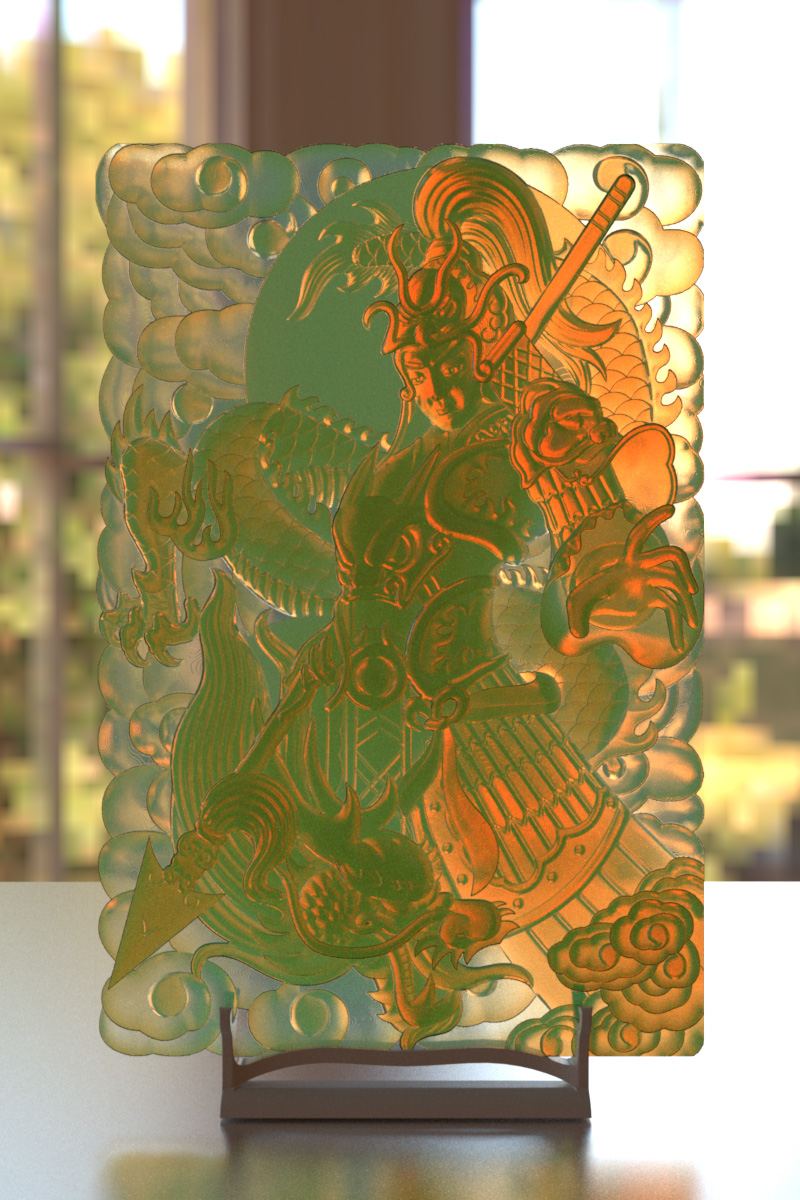
\includegraphics[width=0.24\textwidth]{results/zhaoyun_bg1_1.jpg} &
		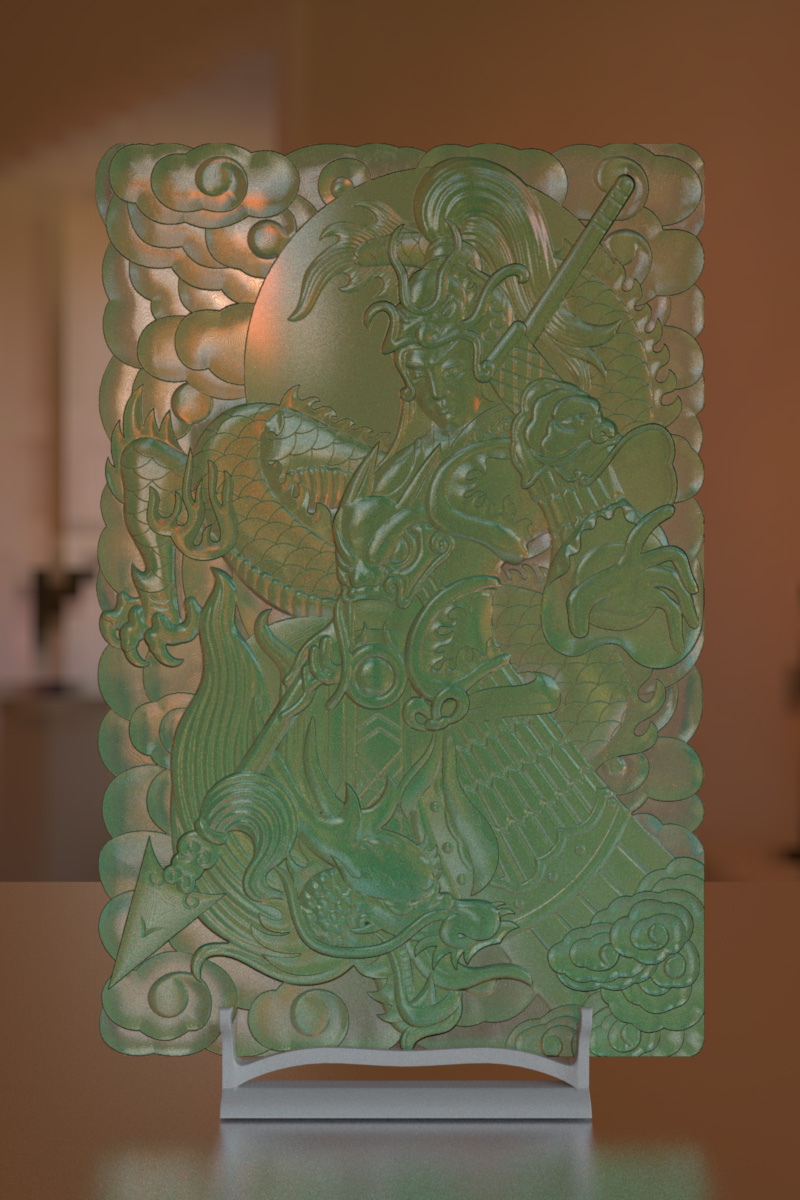
\includegraphics[width=0.24\textwidth]{results/zhaoyun_bg1_2.jpg} &
		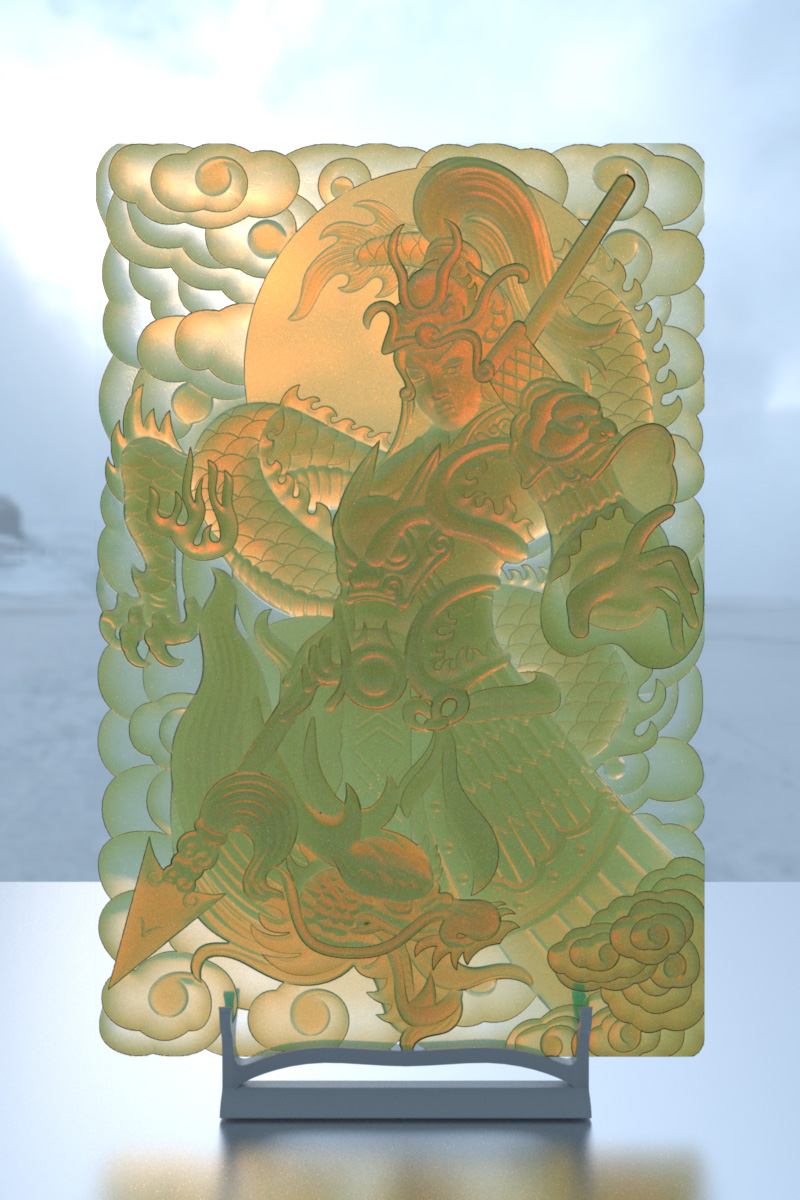
\includegraphics[width=0.24\textwidth]{results/zhaoyun_bg2_1.jpg} &
		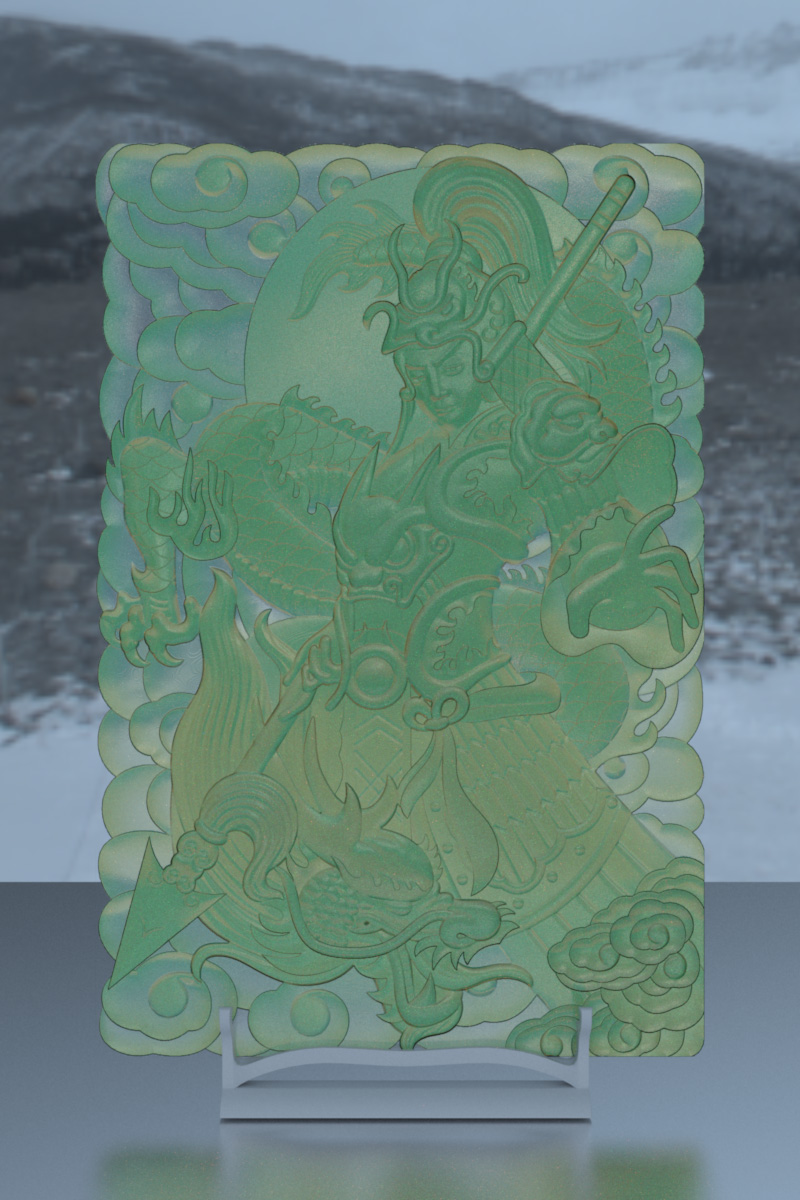
\includegraphics[width=0.24\textwidth]{results/zhaoyun_bg2_2.jpg}\\
		Back-lit & Front-lit & Back-lit & Front-lit
		\\[5pt]
		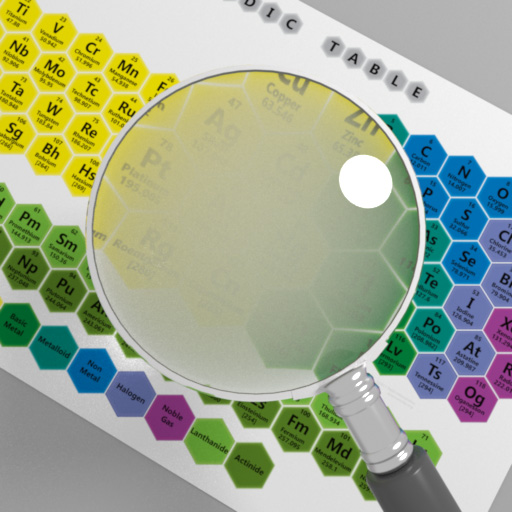
\includegraphics[width=0.24\textwidth]{results/magnify_g9.jpg} &
		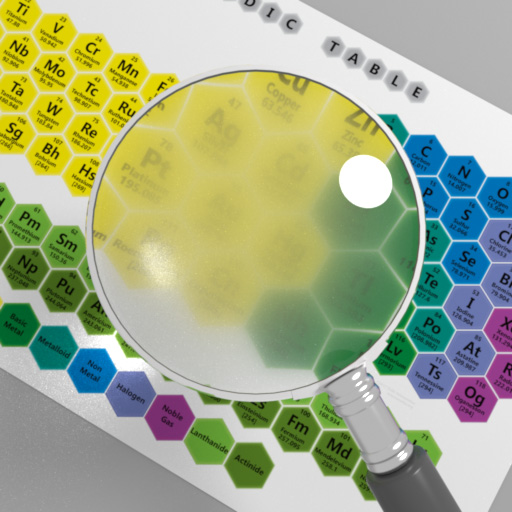
\includegraphics[width=0.24\textwidth]{results/magnify_g99.jpg} &
		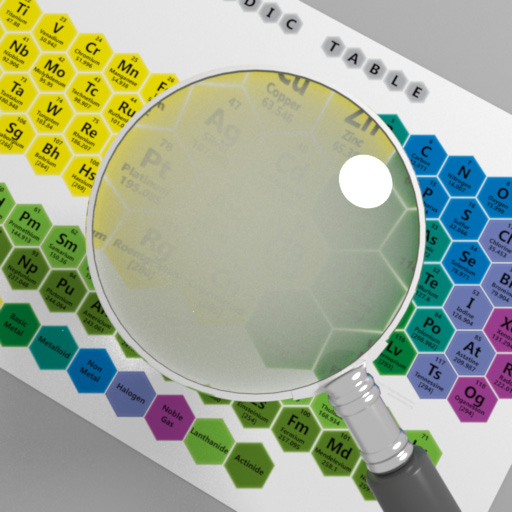
\includegraphics[width=0.24\textwidth]{results/magnify_vmf10.jpg} &
		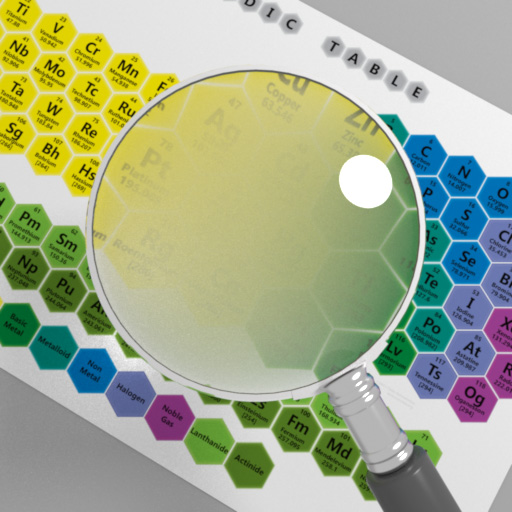
\includegraphics[width=0.24\textwidth]{results/magnify_vmf100.jpg}\\
		HG ($g = 0.9$) & HG ($g = 0.99$) & vMF ($\kappa = 10$) & vMF ($\kappa = 100$)
	\end{tabular}
	%\caption{albedo:0.2,0.95,0.8; $\sigma_t$:1.2,6,12}
	\caption{\label{fig:result_transmit}
		\textbf{Reflection and transmission:}
		Our BSDF models are capable of accurately capturing not only reflection but also transmission from thin layers. \textbf{Top:} A flat surface rendered with our layered BSDF under varying illuminations. This model involves dielectric interfaces with spatially varying roughnesses, normal maps, and thickness. The optical densities (mean free paths) are spectrally varying, which results in subtle color variations across the surface. Note that the color (albedo) is not varying. \textbf{Bottom:} A flat surface with a layered BSDF of spatially varying thickness (which captures the shape of real convex lens). A range of spatially varying and physically plausible blurring effects can be achieved by varying phase functions.
	}
\end{figure*}

\begin{table*}[t]
\centering
	\caption{\label{tab:performance}
		\sz{Render times of all our results (using our ``unidir.'' and ``bidir.'' estimators) as well as baseline models with ``trivial'' BSDFs (that require no stochastic evaluation).
		All the multi-layer models are described using nesting BSDFs for the unidirectional estimator and the explicit implementations for the bidirectional one.
		The baseline models exhibit different appearances and are created solely for performance comparison.
		All the timings are converted to a 6-core Intel i7-6800K CPU time, and those between parentheses indicate render time per mega-pixel.
		The numbers in bold correspond to methods used for creating the paper figures.
		Please refer to the supplemental material for all the other renderings.}
	}
    %
	\begin{tabular}{l|c|c|rr|rr|rr}
	%\hline
	& \multirow{2}{*}{\textbf{Image size}}  & \multirow{2}{*}{\textbf{Spp}} & \multicolumn{6}{c}{\textbf{Render time}}\\
	& & & \multicolumn{2}{c}{\textbf{Unidir.}} & \multicolumn{2}{c}{\textbf{Bidir.}} & \multicolumn{2}{c}{\textbf{Trivial}}\\
	\hline
	\textbf{Fig. \ref{fig:teaser} (a)} & 3000$\times$2000 & 1024           & \sz{2.5 h}  & \sz{(25 m)} & \sz{\textbf{2.2 h}} & \sz{\textbf{(22 m)}}  & \sz{38 m}  & \sz{(6.3 m)}\\
	%\hline
	\textbf{Fig. \ref{fig:result_glints} (b)} & 1024$\times$1024 & 256     & \sz{\textbf{2.2 m}} & \sz{\textbf{(2.1 m)}} & \sz{2.6 m} & \sz{(2.5 m)}   & \sz{1.3 m} & \sz{(1.2 m)}\\
	%\hline
	\textbf{Fig. \ref{fig:result_transmit}, top} & 800$\times$1200  & 512  & \sz{15.2 m}   & \sz{(7.9 m)} & \sz{\textbf{24 m}}  & \sz{\textbf{(12.5 m)}}  & \sz{2.4 m} & \sz{(1.3 m)}\\
	%\hline
	\textbf{Fig. \ref{fig:result_transmit}, bot.} & 512$\times$512   & 1024 & \sz{6.4 m} & \sz{(6.1 m)} & \sz{\textbf{13 m}} & \sz{\textbf{(12.6 m)}}  & \sz{1.6 m} & \sz{(1.5 m)}\\
	%\hline
	\textbf{Fig. \ref{fig:result_mat} (a)} & 876$\times$584   & 256        & \sz{\textbf{1.1 m}} & \sz{\textbf{(2.2 m)}} & \sz{1.4 m} & \sz{(2.7 m)}   & \sz{0.6 m} & \sz{(1.1 m)}\\
	%\hline
	\textbf{Fig. \ref{fig:result_mat} (b)} & 876$\times$584   & 256        & \sz{\textbf{1.1 m}} & \sz{\textbf{(2.2 m)}} & \sz{1.4 m} & \sz{(2.7 m)}   & \sz{0.5 m} & \sz{(0.9 m)}\\
	%\hline
	\textbf{Fig. \ref{fig:result_mat} (c)} & 876$\times$584   & 256        & \sz{\textbf{2.5 m}} & \sz{\textbf{(4.9 m)}} & \sz{5.4 m} & \sz{(10.5 m)}  & \sz{0.5 m} & \sz{(0.9 m)}\\
	%\hline
	\textbf{Fig. \ref{fig:redcloth} (b)} & 640$\times$540   & 256        & \sz{1.5 m}   & \sz{(4.3 m)} & \sz{\textbf{1.9 m}} & \sz{\textbf{(5.5 m)}}   & \sz{0.5 m} & \sz{(1.4 m)}\\
	%\hline
	\textbf{Fig. \ref{fig:result_multilayer} (a)} & 1200$\times$1400 & 256 & \sz{\textbf{6.7 m}}  & \sz{\textbf{(4.0 m)}} & \sz{12 m}  & \sz{(7.1 m)}   & \sz{3.7 m} & \sz{(2.2 m)}\\
	%\hline
	\textbf{Fig. \ref{fig:result_multilayer} (b)} & 1200$\times$1400 & 256 & \sz{\textbf{7.0 m}}  & \sz{\textbf{(4.2 m)}} & \sz{13 m}  & \sz{(7.7 m)}   & \sz{3.7 m} & \sz{(2.2 m)}\\
	%\hline
	\textbf{Fig. \ref{fig:result_multilayer} (c)} & 1200$\times$1400 & 256 & \sz{67 m} & \sz{(40 m)}  & \sz{\textbf{20 m}}  & \sz{(\textbf{12 m})}    & \sz{4.7 m} & \sz{(2.8 m)}\\
	%\hline
	\end{tabular}
	%\\[2pt]
	%\footnotesize{*T/MP: Render time per mega-pixel}
\end{table*}



\subsubsection{Application: Anisotropic layer media for fabrics}
%\myparagraph{Application: Anisotropic layer media for fabrics}
%
Our layered BSDF allows any phase functions within volumetric scattering layers, including anisotropic microflake phase functions~\cite{Jakob:2010:RTF,Zhao:2011:BVA,Heitz:2015:SMD} capable of representing fabrics.
Figure~\ref{fig:result_mat} shows three fabrics modeled using our model with ``null'' top and bottom interfaces (ones that allows light to travel through without reflecting or refracting it) and anisotropic layer media with spatially varying albedo and flake orientations (the optical density does not vary in these examples, though it could).
The satin weave shows well aligned yarns have created smooth and strongly anisotropic highlights. The twill pattern has warp and weft yarns in different colors, leading to dual colored highlights. The velvet exhibits strong grazing-angle highlights, an effect that is challenging to model using traditional BSDF models. Our model successfully captures all the diverse appearances from all three fabrics and produces convincing impressions of these materials.

Figure~\ref{fig:redcloth} shows a fabric rendered using fiber orientation data acquired by micro-CT imaging \cite{Zhao:2011:BVA}. Our rendering uses a fiber orientation map derived from the full data, and matches the full volumetric simulation fairly closely, while being 40 times faster. The speedup is because ours is still a flat BSDF model with parameter mapping, as opposed to full volumetric tracing that requires expensive ray marching through massive data.

\subsubsection{Application: Multiple layers}
%\myparagraph{Application: Multiple layers}
%
Lastly, in Figure~\ref{fig:result_multilayer}, we show rendered results of a kettle with varying layer configurations.
In column~(a), the material has a single transparent water layer with a dielectric interface on the top and a metallic surface on the bottom.
Both interfaces are normal mapped to capture the water drops and the scratches, respectively.
In column~(b), the material shares the same bottom surface as in~(a) but has a smooth top interface and a translucent coating layer with spatially varying optical thickness and albedo, making only part of the bottom surface directly visible.
Lastly, in column~(c), the material has a dual-layer configuration by stacking the layers from~(a) on top of that from~(b).
Our method offers the flexibility to conveniently model all three cases with the last one described using the \sz{explicit implementation} depicted in \S\ref{subsec:multi_layer}.

\subsection{Performance}
%
The Monte Carlo processes for sampling and evaluating our BSDFs do introduce computational overhead.
Table~\ref{tab:performance} lists the performance numbers of all our results.
Further, we provide baseline timings using ``trivial'' BSDFs (that require no stochastic evaluation) to the same scene geometries.
%Without highly scattering medium, rendering with our model is roughly 3$\times$ slower than using standard analytical BSDF models. %(Figure~\todo{XXX}).
Our performance does degrade with the presence of optically thick and highly scattering media.
However, as already demonstrated in Figure~\ref{fig:validation1}, rendering using our model is still significantly faster than explicitly simulating light transport in layered geometries.

\begin{figure*}[t]
	\centering
	\addtolength{\tabcolsep}{-3.5pt}
	\begin{tabular}{ccc}
		\begin{overpic}[width=0.322\textwidth]{img/results/satin_spp128.jpg}
			\put(2,60){\bfseries \color{white} \large (a) Satin}
		\end{overpic}
		&
		\begin{overpic}[width=0.322\textwidth]{img/results/twill_128spp.jpg}
			\put(2,60){\bfseries \color{white} \large (b) Twill}
		\end{overpic}
		&
		\begin{overpic}[width=0.322\textwidth]{img/results/velvet_spp128.jpg}
			\put(2,60){\bfseries \color{white} \large (c) Velvet}
		\end{overpic}
	\end{tabular}
	\caption{\label{fig:result_mat}
		\textbf{Anisotropic media within layers.}
		Our layered BSDF offers the generality to use anisotropic layer media with microflake phase functions.
		This example shows three fabrics modeled with our BSDF model with anisotropic layer media: (a) satin; (b) twill; and (c) velvet.
	}
\end{figure*}    

\begin{figure*}[t]
	\centering
	\addtolength{\tabcolsep}{-3.5pt}
	\begin{tabular}{cccc}
		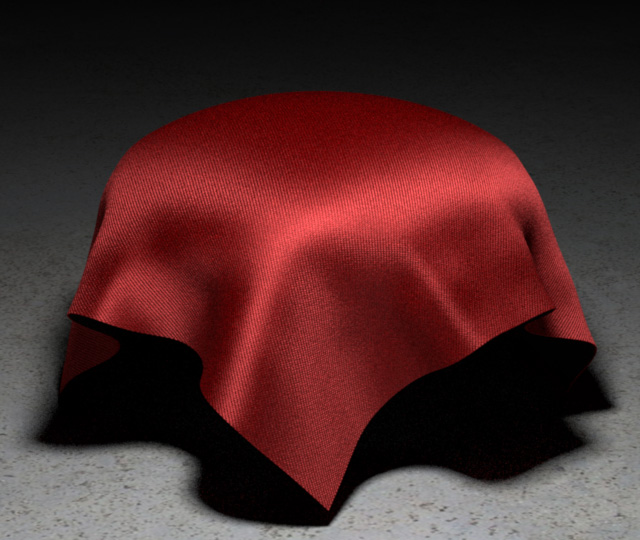
\includegraphics[width=0.24\textwidth]{results/gabardine_ref.jpg} &
		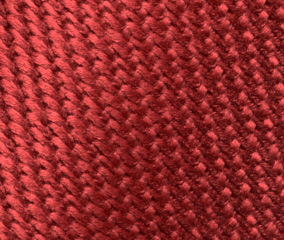
\includegraphics[width=0.24\textwidth]{results/gabardine_ref_inset_128spp.jpg} &
		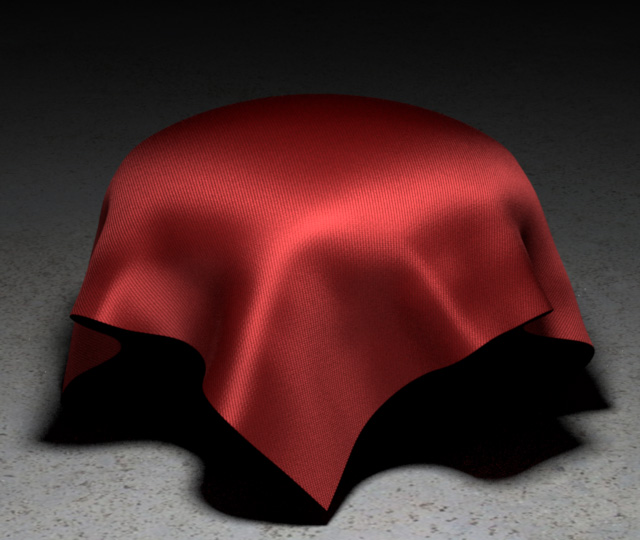
\includegraphics[width=0.24\textwidth]{results/gabardine.jpg} &
		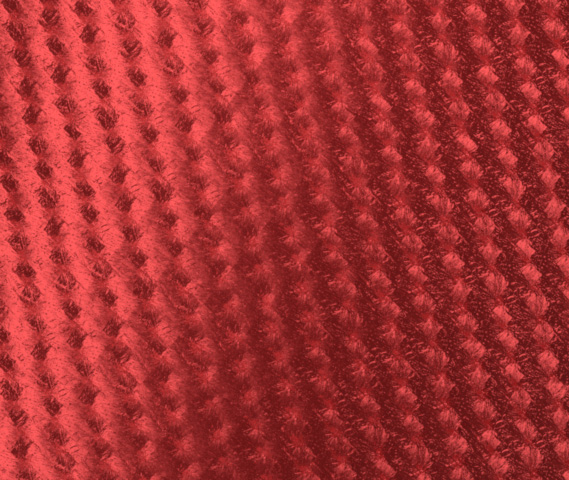
\includegraphics[width=0.24\textwidth]{results/gabardine_inset_512spp.jpg} \\
		\multicolumn{2}{c}{(a) Volume rendering} & \multicolumn{2}{c}{(b) Our BSDF + fiber-direction map}
	\end{tabular}
	\caption{\label{fig:redcloth}
		\textbf{Comparison to volumetric cloth.} \textbf{(a)}~Images rendered from micro-CT volumetric data, using the microflake phase function. \textbf{(b)}~Renderings using our approach using a single microflake volumetric layer, where we are using fiber direction maps extracted from the volumetric data. Our rendering is 40$\times$ faster than the volumetric simulation.
	}
\end{figure*} 


\subsection{Limitations and future work}
\label{subsec:limitation}
%
Our model relies on the assumption of thin flat layers (Figure~\ref{fig:thin_layer}) and cannot capture effects caused by geometric or optical variations at the global scale.
Examples include internal caustics and shadowing arising from major normal variations and color bleeding caused by light scattering though media with varying colors.
Generalizing our technique to include bidirectional subsurface scattering distribution functions (BSSRDFs) is an interesting further topic.
In addition, as our model simulates subsurface scattering using Monte Carlo path tracing, the performance may degrade with the presence of optically thick layers with many scattering events.
Using fast approximated solutions such as~\cite{Jensen:2001:PMS,Frisvad:2014:DDM} to capture multiple scattering may be a useful extension.
Lastly, since we model light transport using traditional radiative transfer, wave effects such as thin film interference are not handled.
An interesting challenge is to integrate wave optics into our model to accurately and efficiently handle light interference and phase shifts.

\begin{figure*}[t]
	\centering
	\addtolength{\tabcolsep}{-3pt}
	\begin{tabular}{ccc}
		\begin{overpic}[width=0.32\textwidth]{img/results/kettle_drop.jpg}
			\put(2,3){\bfseries \color{black} \Large (a)}
		\end{overpic}
		&
		\begin{overpic}[width=0.32\textwidth]{img/results/kettle_logo.jpg}
			\put(2,3){\bfseries \color{black} \Large (b)}
		\end{overpic}
		&
		\begin{overpic}[width=0.32\textwidth]{img/results/kettle_all.jpg}
			\put(2,3){\bfseries \color{black} \Large (c)}
		\end{overpic}
	\end{tabular}
	\caption{\label{fig:result_multilayer}
		\textbf{Multi-layer BSDF.}
		This result shows renderings of a kettle described with: 
		\textbf{(a)}~a single transparent layer with a dielectric top interface capturing the water drops over a conducting bottom surface with scratches; 
		\textbf{(b)}~a single translucent layer with spatially varying optical thicknesses and albedo over the same bottom surface of (a);
		\textbf{(c)}~a dual layer configuration created by stacking the transparent layer~(a) over the translucent one~(b).
	}
\end{figure*}

